\documentclass[12pt,a4paper,english,magyar,oneside]{report}

\usepackage{t1enc}

\usepackage[utf8]{inputenc} % mert nem a középkorban vagyunk
\usepackage[magyar]{babel}
\def\magyarOptions{hyphenation=huhyphn}
\usepackage[style=magyar,natbib=true,babel=other]{biblatex}
\bibliography{bibliography}
%\usepackage{csquotes}
\usepackage{listingsutf8}
\usepackage{color}
\definecolor{lightgray}{rgb}{.9,.9,.9}
\definecolor{darkgray}{rgb}{.4,.4,.4}
\definecolor{purple}{rgb}{0.65, 0.12, 0.82}
%%javascript listing%% 
\lstdefinelanguage{JavaScript}{
  keywords={typeof, new, true, false, catch, function, return, null, catch, switch, var, if, in, while, do, else, case, break},
  keywordstyle=\color{blue}\bfseries,
  ndkeywords={class, export, boolean, throw, implements, import, this},
  ndkeywordstyle=\color{darkgray}\bfseries,
  identifierstyle=\color{black},
  sensitive=\true,
  comment=[l]{//},
  morecomment=[s]{/*}{*/},
  commentstyle=\color{purple}\ttfamily,
  stringstyle=\color{red}\ttfamily %,
  %morestring=[b]',
  %morestring=[b]"
}
\lstset{
   language=JavaScript,
   backgroundcolor=\color{lightgray},
   extendedchars=false,
   basicstyle=\footnotesize\ttfamily,
   showstringspaces=false,
   showspaces=false,
   numbers=left,
   numberstyle=\footnotesize,
   numbersep=5pt,
   tabsize=2,
   breaklines=\true,
   showtabs=\true,
   captionpos=b,
   inputencoding=utf8,
   escapeinside=||
}

%%end of javascript listing%%

\usepackage[T1]{fontenc}

\usepackage{indentfirst} % fejezetek első bekezdését is húzzuk be
\usepackage{lmodern} %szépek lesznek tőle a betűk a pdfben
\usepackage{graphicx}


\usepackage{url}
%\usepackage{subfig}
%\usepackage{times}
% 2.5 centis margó mindenütt, bal oldalt +1 centi kötésnek
\usepackage{anysize}
\paperwidth=21cm \paperheight29.7cm
\marginsize{3.5cm}{2.5cm}{2.5cm}{2.5cm} % {bal}{jobb}{felső}{alsó}
\addtolength\topmargin{-\headheight} \addtolength\topmargin{-\headsep}
\addtolength\textheight{\headheight} \addtolength\textheight{\headsep}
\addtolength\textheight{\footskip}
\footskip=15pt
\ifx\pdfoutput\UnDefined \newcount\pdfoutput \fi
\ifnum0<\pdfoutput
  \pdfpagewidth\paperwidth \pdfpageheight\paperheight \pdfcompresslevel9
\else \special{papersize=21cm,29.7cm} \fi

\sloppy % inkább a térköz nőjön minthogy sorok lógjanak ki jobb szélen

\linespread{1.4} % Másfeles sorköz
\frenchspacing   %Szimpla térköz mondatok között

\usepackage{fancyhdr}
\pagestyle{fancy}

%\usepackage{nomencl} %rovidites jegyzek
%\renewcommand{\nomname}{Rövidítésjegyzék}
%\makenomenclature % roviditesjegyzek

\begin{document}
\selectlanguage{magyar}

% include most passzolva eleg lesz az a vegen is... 
%!TEX root = /Users/oroce/Documents/msc-szakdolgozat/dolgozat.tex
\begin{raggedright}
Budapesti Corvinus Egyetem \\
Gazdálkodástudományi Kar \\
{\small Számítástudomány Tanszék}
\end{raggedright}

\thispagestyle{empty}

\vspace{3.5cm}

\vspace{0.8cm}
\begin{center}
\textbf{\Large SZOLGÁLTATÁSFOLYTONOS ALKALMAZÁSOK MŰKÖDTETÉSE}
\end{center}
% Úgy tűnik az \uppercase nem szereti az ékezetes betűket :(

\vfill
\begin{raggedleft}
Készítette: Oroszi Róbert (\today)\\
Gazdaságinformatikus szak\\
2013\\
\end{raggedleft}
\begin{raggedright}
{\Large Konzulens:}\\ Mohácsi László
\end{raggedright}
\vspace{0.6cm}


\clearpage

%--------------------------------------------------------

%\begin{center}
%\uppercase{Nyilatkozat}
%\end{center}

%\thispagestyle{empty}
%Én, Oroszi Róbert teljes felelősségem tudatában kijelentem, hogy a jelen szakdolgozatban
%szerepelő minden szövegrész, ábra és táblázat – az előírt szabályoknak megfelelően
%hivatkozott részek kivételével – eredeti és kizárólag a saját munkám eredménye, más
%dokumentumra vagy közreműködőre nem támaszkodik.

%\vspace{5 cm}

%\begin{tabular}[h]{c c c}

%Kelt: Budapest, 2011. 05. 02. & \hspace{2cm} & \rule{5cm}{.4pt} \\

% & & Oroszi Róbert

%\end{tabular}

%\clearpage

%\setlength{\parindent}{0.2cm}

 %fedlap

\setcounter{tocdepth}{2} % tartalomjegyzék mélysége
\tableofcontents % tartalomjegyzéks
%\printnomenclature[2.5cm]
%\large{
\chapter{Bevezetés}
%!TEX root = /Users/oroce/Documents/msc-szakdolgozat/dolgozat.tex
Az interneten böngészve a felhasználó gyakran észre sem veszi, de egy weboldalon történő két kattintása között elképzelhető, hogy az adott rendszer kétszer is verziót váltott, azaz frissítette a rendszerét. De hogyan történik mindez? Hogyan lehetséges leállás nélkül naponta többször verziót váltani, akár földrajzilag elosztott rendszereket populálni? Ezekre a kérdésekre kíván a szakdolgozat válaszokat adni.
\\
Bemutatásra kerül a continuous integration folyamat, ezekhez használt rendszerek, eszközök.
\\
A dolgozat témája alapvetően a webes alkalmazásokat hivatott bemutatni, azonban kitér az asztali alkalmazásokra is.
\\
A verzióváltás téma azért rendkívül izgalmas, mert akkor működnek jól, ha a végfelhasználó nem veszi észre, azonban ezeknek a rendszerek megtervezése, kiépítése, működtetése néha komolyabb mérnöki probléma, mint azok az alkalmazások, amelyek számára készültek.


\chapter{Continuous Integration}
%!TEX root = /Users/oroce/Documents/msc-szakdolgozat/dolgozat.tex
\begin{quotation}
A Continuous Integration - azaz a folyamatos integráció - egy olyan szoftverfejlesztési módszertan, amelyben a fejlesztőcsapat tagjai által írt kód napi rendszerességgel kerül (vagy automatizálással minden funkció, javítás implementálása után) integrálásra a korábbi fejlesztések közé. Minden új kód integrálása során automatizált tesztek ellenőrzik, hogy a rendszerbe való illesztés során okozott-e valamilyen hibát az új kódrészlet, illetve megfelel-e az adott fejlesztőcsapat által meghatározott minőségi kritériumoknak és ennek eredményéről a lehető leghamarabb visszajelzést ad. \cite{martin_fowler_cont_int}
\end{quotation} 

A szoftverfejlesztés során általában egy projekten több fejlesztő is dolgozik a kód különböző vagy akár egyazon részein is. A fejlesztők az alkalmazás másolatával dolgoznak a saját munkaállomásukon (nem pedig közvetlenül egy helyen). Ha egy feladat elkészül, akkor fel kell másolni a módosított fájlokat egy közös tárolóba/szerverre. Viszont a felmásolás előtt mindenképpen szükséges frissíteni a saját lokális példányukat, hogy elkerüljék a ütközéseket, illetve egymás munkájának felülírását, ezt a folyamatot nevezik integrációnak. Azonban előfordulhat, hogy a központi tároló és a saját lokális másolat között akkora különbség lehet, hogy nagy mértékben kénytelen a fejlesztő módosítani a saját fejlesztését, majd a javítás elvégzése után következhet ismét egy frissítés (integrálás), majd esetleg a megismételt javítás. Ez mint látható, egy ördögi kör. Ennek a megoldására jött létre a Continuous Integration, amelynek segítségével a fejlesztők adott időközönként megismétlik az integrációs lépést, hogy minél kevésbé térjen el a lokális verzió a központi tárolóban lévő verziótól.
\hfill\\
Hiába tűnik ez egy triviális és egyszerű megoldásnak, ez a megközelítés csak a 2000-es évek elején született meg, viszont azóta töretlen népszerűségnek örvend. Mára a folyamatos integráció összekapcsolódott az automatikus fordítással (build automation), azonban alapvetően nem szükséges része. Tehát például egy céges előírás, amely megköveteli, hogy a fejlesztők kötelesek minden reggel frissítsék a lokális másolatuk frissítésére, tulajdonképpen folyamatos integrációnak tekinthető, mert ezáltal megvalósítják a rendszeres integrációt. Ezek alapján kijelenthető, hogy a Continuous Integration valójában csak egy verziókezelő (pl.: git, Subversion, Mercurial) használatát követeli meg.
\\
Az automatizált fordítás, habár nem alapvető része a folyamatos integrációnak mégis a fejlesztést és a fejlesztők munkáját nagyban megkönnyíti. Ez a művelet történhet bizonyos időközönként (munkaidő után éjszaka) vagy bizonyos események során, mint például ha fejlesztők feltöltik a közös tárolóba a fájljaikat (commit). Az integrációs lépések és az automatikus fordítás közé érdemes lehet beépíteni a kódminőség ellenőrzést és a tesztelést, amely garantálja, hogy az új funkciók nem törik el a régi funkciókat. Továbbá érdemes az integrációról, a tesztelésről, és a fordításról riportokat generálni, melyekkel az eredmények - egy nem fejlesztő számára is - érthetőbb formába kerülnek.
\\
A folyamatos integrációra, kódminőség ellenőrzésre, tesztesetek futtatására, riportok értelmezésére már sok szoftver elérhető, többek között a Bamboo, amely a Jira és az Confluence mögött álló Atlassian terméke, vagy a Travic CI, amely ingyenes szolgáltatásként elérhető bármilyen nyílt forráskódú szoftver számára, illetve a mára de-facto rendszernek tekinthető Jenkins, amely a következő fejezetben kerül bemutatásra.

\section{Jenkins\\\small{https://jenkins-ci.org/}}
A Jenkins egy ingyenesen elérhető, nyílt forráskódú folytonos integráció támogató eszköz. A legtöbb verziókezelő rendszert támogatja, és több mint 300 kiegészítő érhető el hozzá, melyek segítségével könnyedén testreszabható. A legnagyobb előnye, és amiért az iparági sztenderddé válhatott, az az, hogy rendkívül moduláris, könnyen konfigurálható és képes kiszolgálni egy egyéni projekt és egy nagyobb cég igényeit is.\hfill\\
A legtöbb platformra (Windows, Linux disztribúciók, OSX, BSD) elérhető szoftver, amellett hogy nyílt forráskódú kereskedelmi támogatással is rendelkezik.\hfill\\
Azon túl, hogy a folyamatos integráció lépések sorozatába rendezhető, melyet a webes felületen keresztül, konfigurációs fájl vagy akár szakterület-specifikus nyelv (DSL) használatával is testre szabható a létrehozott feladatok (job) egymásba is integrálhatóak, a függőségi viszony (upstream, downstream) meghatározásával.\hfill\\
A kiegészítők segítségével testreszabható a bemeneteli forrás (verziókezelők, lokális mappa), az indítási jelzés (start gomb megnyomása, a tárolóba való feltöltés, a programozható interfészen keresztüli hívás, a szülőfeladat állapotváltozása), a kódminőségellenőrzés (checkstyle, linting), a kód építése (ant, grails, gradle), a tesztek lefuttatása (xUnit, TAP) és eredményük analizálása, majd továbbításuk további rendszerekbe (tesztekkel lefedett kód százalékos változása a kód átnézést kezelő rendszerbe, az eltört tesztekről email értesítés) és egyéb szervezet specifikus értesítés kiküldése (release manager értesítése, a különbséget beküldő értesítése).
Amint látható, a Jenkins képes alkalmazkodni a szervezetek által felállított igényekhez, technológiákhoz, ennek is köszönhető töretlen népszerűsége mind a vállalati, mind az open source világban.

\section{TDD\\\small{Test Driven Development}}
A folyamatos integráció és az automatikus fordítás egyik legfontosabb velejáró kulcsszava a TDD, azaz a teszt vezérelt fejlesztés.
\\
A TDD használatához egy elég erős szemléletváltásra van szükség, ezért legalább annyi ellenzője van, mint támogatója. A teszt vezérelt vagy teszt irányított fejlesztés a nevével ellentétben nem egy tesztelési megoldás, hanem sokkal inkább tervezési. \cite{tddjs_definition}
\\
Egy alkalmazás jó és jól működéséhez könnyen bővíthetőnek kell lennie, így tud a termék, szolgáltatás megújulni, a továbbfejlesztés zökkenőmentesen zajlani. De hogyan történik az új funkciók tervezése, beépíthetőségi megvalósításának tervezése?
\\
A TDD ezt próbálja elősegíteni azáltal, hogy a teszteseteket még a tervezés fázisában kell megírni, így a problémák a munka korai fázisában kiderülhetnek. A TDD keretrendszerek általában könnyen olvashatóak még a fejlesztésben kevésbé járatos projektrésztvevők számára is, \aref{fig:mocha_should_tdd_test} ábra ezt kívánja bemutatni.
\ref{fig:mocha_should_tdd_test}
\begin{figure}[H]
	\centering
		\lstinputlisting[language=Javascript]{assets/mocha_test.js}
		\caption{Egy TDD teszt mocha és should keretrendszerekkel}
		\label{fig:mocha_should_tdd_test}
\end{figure}
\hfill\\
Mivel a TDD teszteseteket a fejlesztés alatt folyamatosan futtatják - ellenben az egységtesztekkel, melyek általában az integráció során futnak le -, ezért kimondottan gyorsnak, mindenhol, bármilyen sorrendben futtathatónak kell lenniük, mert egyébként a fejlesztők nem fogják felhasználni őket. Teszteseteknek csak akkor kellene változniuk, ha a kód ezt megköveteli, illetve ha a specifikáció változik.
\hfill\\
A fejlesztési folyamat négy lépésre bontható:
\hfill\\
\begin{description}
\item[Feladatok meghatározása]\hfill\\
     Ebben a lépésben az ügyfél igényeknek megfelelő funkcionalitást kell összegyűjteni tesztesetek formájában, és meg kell határozni, hogy mit kellene tennie a rendszernek.\hfill\\
     Fontos, hogy nem azt kell itt kitalálni, hogy az adott fejlesztő hogyan valósítsa meg az adott feladatot, hanem hogy mit kell majd megvalósítani. A "mit" meghatározása által a fejlesztő is jobban megérti a feladatot, így kisebb a félreértés lehetősége. A teszteset megírása után következik a megvalósítás.
\hfill\\
\item[Megvalósítás]\hfill\\
     A tesztesetek elkészültével következik az előre specifikált feladat megvalósításának megtervezése, melyet a megvalósítás követ.\hfill\\
     A megvalósításnak kellene a legkönnyebb résznek lennie, ha mégsem könnyű, akkor a következő problémák fordulhattak elő. \\
Túl nagy feladat került meghatározásra az előző lépésben, így a következő lépésben az adott feladat kisebb részfolyamatokra bontásának kell megtörténnie.\\
Felmerül a kérdés, hogyan lehet könnyű a megvalósítás, ha előtte még egy alkotóelemet is el kell készíteni? Ilyenkor az adott alkotóelem feladatait kell meghatározni úgy, hogy a fejlesztők lesznek az ügyfelek és a ő igényeiket kell kielégíteni, és TDD alapján lefejleszteni.\\
Ha nem nagy lépésről van szó, de mégis nehéz megvalósítani, akkor refaktorálni kell az adott részt. Ezt okozhatja az, hogy koszos a kód, vagy nincs jól megtervezve. A refaktorálást a már korábban megvalósított tesztesetek teszik lehetővé, melyek biztosítják, hogy a kódújraszervezés során nem fog eltörni egyik korábbi vagy jövőbeni komponens sem.
\hfill\\
\item[Ellenőrzés]\hfill\\
     A megfelelő eszközzel le kell ellenőrizni, hogy sikeresek lettek-e a tesztek. Ennek gyorsnak és könnyűnek kell lennie. (A tesztek nem futhatnak néhány másodpercnél lassabban.) Ezáltal folyamatosan ellenőrzött, tervezett és fejlesztett lesz a kód.
\hfill\\
\item[Tisztítás]\hfill\\
Ha sikeresen le lehet futtatni a teszteket, akkor következik a kód tisztítása. A működő kódot át kell nézi, a duplikációkat eltüntetni.\\Ajánlott beszédesebb neveket választani a változóknak, a függvények hosszát érdemes csökkenteni kiszervezés segítségével, újrafelhasználhatóság szem előtt tartása mellett. Mivel az ügyfél számára fontos funkcionalitás már le van tesztelve, ez a művelet már könnyedén elvégezhető, ugyanis ha például egy metódus neve elgépelésre kerül, akkor rögtön jelez a teszt, hogy hiba van. Ettől tisztább és karbantarthatóbb lesz a kód.
\end{description}

Érdemes megfigyelni, hogy az összes lépés megfeleltethető a tervezés egy-egy részének. A meghatározott feladatok automatizálásának köszönhetően lehetséges, hogy kis, biztonságos, önellenőrzött lépésekben történjen a rendszer felépítése és tervezése. Ez segíti a feladat megértését, rákényszerít az átlátható megvalósíthatóságra a folyamatos tisztítás és az újratervezés segítségével.\\
\hfill\\
\textbf{TDD előnyei:}

\begin{itemize}
\item Refaktorálást segíti.
\item A kód módosítása könnyebb, hiszen hiba esetén a tesztek eltörnek, amely azonnali visszacsatolást ad a fejlesztő számára.
\item Könnyebb egy tesztelhető kódot refaktorálni (a tervezés miatt).
\item Az is segítség lehet, hogy hol nincs hiba.
\item Segít tesztelhetővé tenni az alkalmazást.
\item Rákényszerít, hogy ne legyen az alkalmazásban spagetti kód\nomenclature{spagetti kód}{\hfill\\A kifejezést olyan programkódra használják pejoratív értelemben, amelyek komplex vagy kevésbé komplex feladatot struktúrálatlanul, átláthatatlanul oldalanak meg.}.
\item Felesleges funkció nem kerül megvalósításra, csak az, ami a teszthez szükséges.
\item Előre kell tervezni.
\item Gyors, folyamatos visszajelzés kapható a funkció állapotáról (nem csak az adott fejlesztőknek, de a csapat többi tagjának és a projektmenedzsernek is).
\item Jobban ellenőrizhető a munka.
\item Van, hogy egy funkciónak nincs látható eredménye egy hétig. Ezzel szemben a TDD-nél naponta meg lehet mondani, hogy mennyi sikeres tesztet sikerült írni.
\item Segít megérteni a feladatot a példákon keresztül.
\item Időcsökkentő tényező a hibajavításnál és a refaktorálásnál.
\item Hibajavításnál segíthet pontosabban megjelölni a hiba helyét.
\item Akár dokumentációként is szolgálhat a teszt.
\item Biztosítja, hogy az új kód nem érint más tesztelt egységet.
\item Ha nincs TDD, akkor gyorsabban készül a szoftver, de nehezebben módosítható később.
\item A TDD tisztítás része akár kódfelülvizsgálatnak is tekinthető.
\item Stabilitást elősegítheti.
\item Segíti a kódstrukturálást, megköveteli a modularizációt, mert egyébként a teszt megírása bonyolultabbá válik, mint a tesztelendő kód.
\end{itemize}
\hfill\\
\textbf{TDD hátrányai:}

\begin{itemize}
\item Nő a fejlesztési idő (refaktorálásnál csökken).
\item Ha nem tiszta, hogy mit kell tenni az adott feladattal, könnyen előfordulhat, hogy rossz teszt kerül megírásra, amit át kell majd írni. (Újabb időnövelő tényező.)
\item Menet közben történt koncepcióváltásnál ki kell dobni a teszteket. (Újabb időnövelő tényező.)
\item A program működése nem lesz hibamentes, ha a tesztek sikeres lefutnak.
\item Nem csodafegyver. A rendszer tesztelésének (minőségbiztosításának) csak egy kis részét képezi (egységtesztelés, elfogadási tesztelés, integrációs tesztelés, regressziós tesztelés mellett).
\item Csak tapasztalt fejlesztőkkel érdemes használni.
\item A tervezést nem mindig lehet úgy alakítani, hogy az megfeleljen a TDD-nek.
\item Hálózati műveleteket, fájlrendszert igénylő komponensek tesztlésére nem ajánlott.
\item Páros programozásban a legjobb használni, mert így a tesztírás és az implementáció jól felosztható.
\item A tesztek írása unalmas lehet egyesek számára. Nagy fegyelemre van szükség.
\item Nehéz belerázódni, ezért arra a következtetésre lehet jutni, hogy semmi értelme.
\item Nehéz megmagyarázni a menedzsereknek/ügyfeleknek, hogy az elején, a fejlesztés első lépéseinél miért van szükség a többletidőre, miközben látható eredmény nem készül.
\end{itemize}

Az automatizált tesztekkel és azok folyamatos futtatásával a szervezet folyamatosan képet kaphat arról, hogy az implementáció lépései hol tartanak, a folyamatos visszajelzések már előre tudják értesíteni a döntési pozícióban lévő szereplőket, így azok információhiánya csökkenthető. Továbbá egy olyan környezet, ahol a folyamatos integráció gyakorlata használatban van, a felmerülő problémák esetén be tudja építeni az automatizált ellenőrzések közé a problémák megoldásából megszülető újabb ellenőrzéseket, amellyel meg tudja előzni, hogy ismét elkövesse ugyanazt a hibát.
\\
A dolgozat a folyamatos integráción belül is csak a tesztvezérelt fejlesztéssel foglalkozik, de természetesen az egységtesztek, az integrációs tesztek is teljesértékű részei a folyamatnak, viszont míg az utóbbiakat a szervezetek többsége használja addig mindez a TDD-ről nem mondható el, ezért került az kiemelésre és megvizsgálásra.

\section{Webes alkalmazások}
%!TEX root = /Users/oroce/Documents/msc-szakdolgozat/dolgozat.tex
A webes alkalmazásoknál a folyamatos integráció több feladatot is ellát:
\begin{itemize}
	\item tesztek futtatása (unit, tdd, bdd, acceptance, integration)
	\item a fő verzióba való olvasztás
	\item adatbázis migrációs fájlok létrehozása
	\item kliensoldali statikus tartalmak konkatenálása, minimalizálása
\end{itemize}

A közösségi kódmegosztó github integrációs folyamata teljesen megfelel a felsorolásnak (\cite{github_deployment_web}). A különbség mindössze annyi, hogy miután sikeresek a continuous integration lépései egyből élesítésre kerülnek, azaz a fejlesztők a felelősek, ha valami hibát vétenek egy-egy funkció implementálásában.

Viszont a Facebook a saját PHP-ban írt alkalmazásának performancia javításának céljából további feladatokat is végez a folyamatos integrálás során, ez pedig a buildelés. A buildelés során a Facebook saját kódbázisát transzformálja amelynek köszönhetően hatszoros gyorsulást sikerült elérniük (a PHP kódot optimalizált C kódra alakítják, az átalakítás során használt szoftver \href{https://github.com/facebook/hiphop-php}{ingyenes elérhető}). \cite{facebook_deployment}
\subsubsection{Tesztek futtatása}
A tesztek futtatása a webes rendszerekben ugyanolyan fontos, mint bármelyik másik platformon. Viszont míg az asztali és mobil alkalmazásoknál, ismerhető a kliensek rendszer tulajdonságai (például ha egy alkalmazás csak Windows 7 operációs, akkor tudni lehet az azon elérhető futtathatósági lehetőségeket), azonban a webes alkalmazásoknál az nem csak különböző operációs rendszerekre kell optimalizálni, hanem az eltérő böngészőkre (melyek a lehető legkülönbözőbb módon implementálták az egyébként is laza HTML és ECMAScript szabványokat) és azok különböző verzióra. Ezeknek az okoknak köszönhetően a tesztelés, illetve a tesztautomatizálás rendkívül fontos a webes alkalmazásoknál (\cite{tddjs}).

\subsubsection{Kliensoldali tartalmak}
A kliensoldali tartalmak konkatenálása és minimalizálás rendkívül fontos webes alkalmazásoknál, ugyanis ezek a statikus tartalmak - a HTML mellett - az alkalmazás minden betöltésekor letöltésre kerülnek, ami pedig sok különálló fájl esetén a felhasználó élmény rovására mehet.


\section{Asztali alkalmazások}
%!TEX root = /Users/oroce/Documents/msc-szakdolgozat/dolgozat.tex

Az asztali alkalmazások esetén az alkalmazások frissen tartása, frissítése egy bonyolultabb folyamat, mert míg a webes alkalmazásoknál az új verzió elhelyezését, élesítését az alkalmazás fejlesztője - vagy PaaS esetén egy harmadik fél - végzi, addig az asztali alkalmazásoknál, a frissítés végbemenetele a végfelhasználó részéről interakciót igényel.
\hfill\\
Az asztali alkalmazások frissítésére egy tökéletes példa a Google Chrome. Ahogyan \aref{fig:statcounter_browser} ábrán látható, a keresőóriás Google böngészője már 2012. decemberében már legelterjedtebb böngésző volt. Azonban a Chrome verzióváltási politikája elég erőteljesen eltér az iparban megszokottól, mert minden hatodik héten új verziót adnak ki (\cite{chrome_six_weeks}) és emellett a szoftver automatikusan ellenőrzi, hogy van-e elérhető frissítés és amennyiben rendelkezésre áll új verzió, akkor automatikusan letöltésre kerül (\cite{google_chrome_autoupdate}).

\begin{figure}[ht]
	\centering
		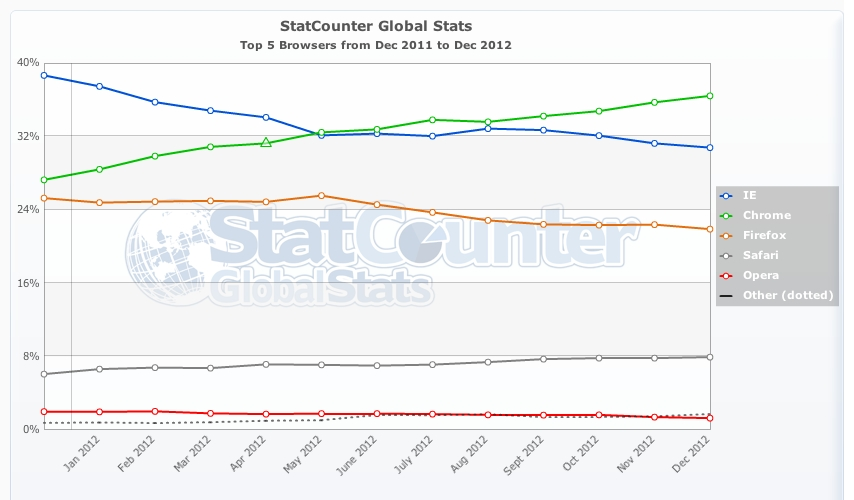
\includegraphics[scale=0.5]{assets/statcounter_browser_2011_dec-2012_dec.jpg}%
		\caption[DUMMY]%
		{Böngészők piaci részesedése 2011. december és 2012. decembere között (\cite{statcounter_browser})}%
		\label{fig:statcounter_browser}
\end{figure}

Azonban más cégek, mint például a github, nem hat hetente ad ki új verziót, hanem a négy hónap alatt huszonöt új verziót tettek elérhetővé (\cite{github_deployment_windows}). Ilyen gyakori kiadási ciklus, csak úgy valósítható meg, ha a legtöbb folyamat automatizálásra kerül (mint ahogy a github automatizálja is), mert ezáltal szinte kizárják az emberi hanyagság okozta hibákat, illetve erőforrást képesek spórolni.




%\section{Okostelefon alkalmazások}
%%!TEX root = /Users/oroce/Documents/msc-szakdolgozat/dolgozat.tex

\cite{linkedin_mobile_deployment}

\subsection{iOS}
\cite{jenkins_ios_deployment}

\subsection{Android}
\cite{jenkins_android_deployment}

\newpage

\printbibliography


%}
\end{document}

